\documentclass{article}
\usepackage{stocktonmacros} % Personal macros, import package
\setlist[itemize]{noitemsep, topsep=0pt} % Must keep within the same document as \begin{document}

\begin{document}

\maketitle
%
\newpage
%
\tableofcontents
%%
\newpage
%%
\import{Lectures/}{Partial Differential Equations - An Introduction}
\import{Lectures/}{Heat, Wave Equation}
\import{Lectures/}{Approximating Functions with Other Functions}
\import{Lectures/}{Heat Equation}
\import{Lectures/}{Wave Equation}
\import{Lectures/}{Boundary Conditions}
\import{Lectures/}{Laplace's Equation}
\import{Lectures/}{Polar Coordinates}
\import{Lectures/}{Complex Analysis, Fourier Transform}
\import{Lectures/}{Transport Equation}
\import{Lectures/}{Image Processing}
\import{Lectures/}{Conservation Laws}
\import{Lectures/}{Exam 2 Review}
%______________________________________________________________________________%
\newpage
% Conservation Law?
\subsection{Traffic Flow}
\topic{April 11, 2022}
Conservation of Cars

Traffic in - Traffic out = Accumulated traffic

\begin{center}
  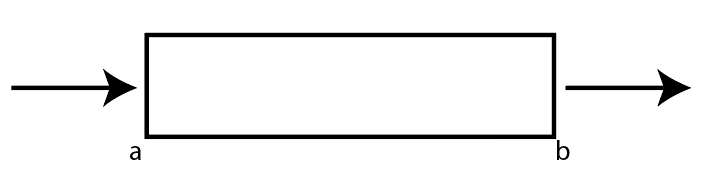
\includegraphics{Conservation Laws - Traffic Flow 1}
\end{center}

Let $\rho(x, t)$ be the density and $q(x, t)$ is the flux.
%
\begin{align}
  \frac{d}{dt} \int^b_a \rho(x, t)\ \text dx
  & = q(a, t) - q(b, t)\\
  & = -\int^b_a q_x (x, t)\ \text dx\\
  \int^b_a (\rho_t + q_x)\ \text dx & = 0\\
  \rho_t + q_x & = 0
\end{align}

Here, $u$ is car velocity:
%
\begin{align}
  q & = pu
\end{align}

Now,
%
\begin{align}
  \rho_t + [\rho u]_x & = 0
\end{align}

Both $\rho$ and $u$ are a function of $x$, therefore there is a product rule that comes into play.
%
\begin{align}
  \rho_t + [c(\rho)]\rho_x & = 0
\end{align}

We have yet to determine $c$. So far, this equation is similar to the Transport Equation, where we use $c$ to find the speed of the equation.

$c(\rho)$ will give the speed of the characteristic.

In general, the car velocity should be a decreasing function of $\rho$.

When $\rho = 0$, the car moves the fastest $= u_{\text{max}}$

When $\rho = \rho_{\text{max}} \Rightarrow u = 0$

The simplest relationship which satisfies these is:
%
\begin{align}
  u(\rho) & = u_{\text{max}}\left(1 - \frac{\rho}{\rho_{\text{max}}}\right)
\end{align}

This tells me,
%
\begin{align}
  q(\rho)
  & = u_{\text{max}} \rho\left( 1 - \frac{\rho}{\rho_{\text{max}}}\right)\\
  & = u_{\text{max}} \rho - \frac{u_{\text{max}}}{\rho_{\text{max}}} \rho^2
\end{align}

Hit maximum velocity at $\frac{\rho_{text{max}}}{2}$
%
\begin{align}
  q_x
  & = u_{\text{max}} \rho_x - 2 \frac{u_{\max}}{\rho_{\max}} \rho \rho_x\\
  & = u_{\max} \left[ 1 - \frac{2}{\rho_{\max}} \rho \right] \rho_x
\end{align}

Here, this shows our critical point is at $\frac{\rho_{\max}}{2}$. Let us redefine this equation as $c(\rho) \rho_x$.
%
\begin{align}
  \rho_t + u_{\max} \left( 1 - \frac{2\rho}{\rho_{\max}}\right) \rho_x & = 0
\end{align}

\ex When a red light turns green.
%
\begin{align}
  \rho(x, t) & =
  \begin{cases}
    \rho_{\max} & x < 0\\
    0 & x > 0
  \end{cases}
\end{align}

Recall, the speed of our characteristic:
%
\begin{align}
  c(\rho) & = u_{\max} \left(1 - \frac{2 \rho}{\rho_{\max}}\right)
\end{align}

The slope of our characteristic is:
%
\begin{align}
  & = \frac{1}{u_{\max} \left(1 - \frac{2 \rho}{\rho_{\max}}\right)}
\end{align}

When we have $\rho = \rho_{\max}$, our slope is $- \frac{1}{u_{\max}}$.

When we have $\rho = 0$, our slope is $\frac{1}{u_{\max}}$.
%
\begin{align}
  \rho(x, t) & =
  \begin{cases}
    \rho_{\max} & x < - u_{\max} t\\
    \frac{\rho_{\max}}{2} \left(1 - \frac{x}{u_{\max}t}\right)
    & -u_{\max} t < x < u_{\max} t\\
    0 & x > u_{\max} t
  \end{cases}
\end{align}

\ex When the light turns red, hit bumper-to-bumper traffic.

For $x < 0$, we have $\rho(x, 0) = \rho_0$.

For $x > 0$, we have $\rho(x, 0) = \rho_{\max}$.

Here, let us write:
%
\begin{align}
  u_t + [f(u)]_x & = 0\\
  \xi^\prime(\aleph) & = \frac{f(u_L) - f(u_R)}{u_L - u_R}
\end{align}

Our $q$ is:
%
\begin{align}
  q(\rho) = u_{\max} \rho\left(1 - \frac{\rho}{\rho_{\max}}\right)
\end{align}

If we consider our graph, a shock will form and we will have:
%
\begin{align}
  \xi^\prime(t) & = \frac{q(\rho_L) - q(\rho_R)}{\rho_L - \rho_R}\\
  & = \frac{u_{\max} \rho_0 \left( 1 - \frac{\rho_0}{\rho_{\max} - 0}\right)}{\rho_0 - \rho_{\max}} < 0
\end{align}
\end{document}
